%vim: ft=tex
%!TEX encoding = UTF-8 Unicode
\documentclass[12pt,french]{article}

\input{../../commons.tex.inc}

\title{Exercices lois de probabilités}
\date{mai \the\year}
\author{Bac 2015}

\SetupExSheets{headings=block-subtitle}

\begin{document}

\maketitle

\begin{question}[subtitle={Pondichery 2015}]
Des études statistiques ont permis de modéliser la durée de vie, en mois,
d'un type de lave-vaisselle par une variable aléatoire $X$ suivant une loi
normale $\mathcal{N}\left(\mu,~ \sigma^2\right)$ de moyenne $\mu = 84$ et
d'écart-type $\sigma$. De plus, on a $P(X \leqslant 64) = 0,16$.

La représentation graphique de la fonction densité de probabilité de $X$ est
donnée ci-dessous.

\begin{center}
  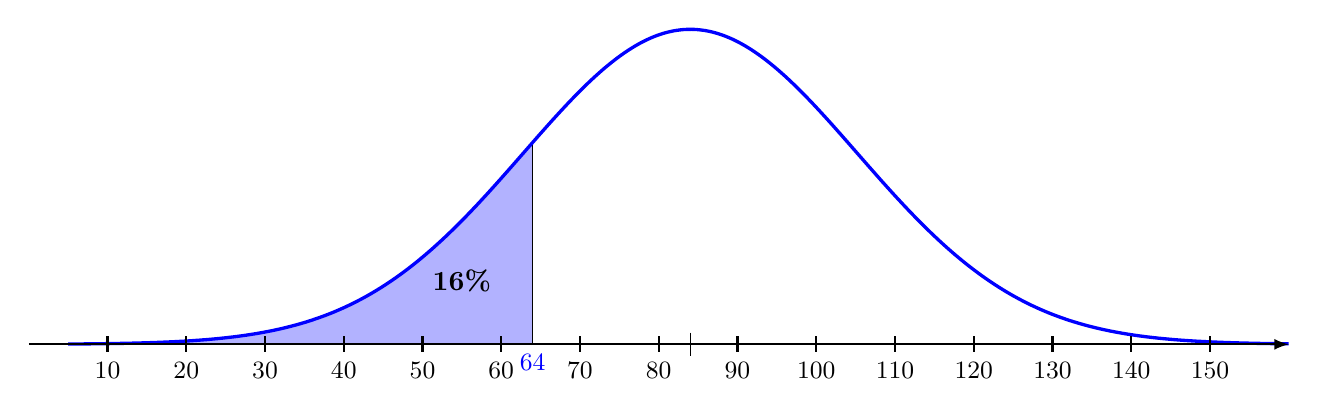
\begin{tikzpicture}[xscale=0.1,yscale=4,>=latex]
    \fill [blue!30] plot [samples=500,domain=5:64] (\x,{exp(-(\x -
    84)^2/900)}) -- (64,0) -- cycle ;
    \draw (64,{exp(-(64-84)^2/900)}) -- (64,0) node [below,blue] {\small 64}
    ;
    \draw [very thick, blue] plot [smooth,samples=500,domain=5:160]
    (\x,{exp(-(\x - 84)^2/900)}) ;
    \draw (55,0.20) node {\bf 16\%} ;
    \draw [thick,->] (0,0) -- (160,0) ;
    \foreach \x in {10,20,...,150} {
      \draw[thick] (\x,0.025) -- (\x,-0.025) node [below] {\small \x} ;
    }
    \draw (84,0.0375) -- (84,-0.0375) ;
  \end{tikzpicture}
\end{center}

\begin{enumerate}
  \item 
    \begin{enumerate}
      \item En exploitant le graphique, déterminer $P(64 \leqslant X
        \leqslant 104)$.
      \item Quelle valeur approchée entière de $\sigma$ peut-on proposer ?
    \end{enumerate}
  \item On note $Z$ la variable aléatoire définie par $Z = \dfrac{X -
    84}{\sigma}$.
    \begin{enumerate}
      \item Quelle est la loi de probabilité suivie par $Z$ ?
      \item Justifier que $P(X \leqslant 64) = P \left(Z \leqslant \dfrac{-
        20}{\sigma}\right)$.
      \item En déduire la valeur de $\sigma$, arrondie à $10^{-3}$.
    \end{enumerate}
  \item Dans cette question, on considère que $\sigma = 20,1$.

    Les probabilités demandées seront arrondies à $10^{-3}$.
    \begin{enumerate}
      \item Calculer la probabilité que la durée de vie du lave-vaisselle
        soit comprise entre 2 et 5~ans.
      \item Calculer la probabilité que le lave-vaisselle ait une durée de
        vie supérieure à 10 ans.
    \end{enumerate}
\end{enumerate}
\end{question}

\begin{question}[subtitle={Amérique du Nord 2015}]
Une entreprise fabrique des tablettes de chocolat de 100~grammes. Le service
de contrôle qualité effectue plusieurs types de contrôle. 

\bigskip

\textbf{Partie A Contrôle avant la mise sur le marché}

\medskip
 

Une tablette de chocolat doit peser 100 grammes avec une tolérance de deux
grammes en plus ou en moins. Elle est donc mise sur le marché si sa masse
est comprise entre 98 et 102 grammes. 

La masse (exprimée en grammes) d'une tablette de chocolat peut être
modélisée par une variable aléatoire $X$ suivant la loi normale d'espérance
$\mu = 100$ et d'écart-type $\sigma = 1$. Le réglage des machines de la
chaîne de fabrication permet de modifier la valeur de $\sigma$.

\medskip

\begin{enumerate}
  \item Calculer la probabilité de l'évènement $M$ : \og la tablette est
    mise sur le marché \fg. 
  \item On souhaite modifier le réglage des machines de telle sorte que la
    probabilité de cet évènement atteigne 0,97. 

    Déterminer la valeur de $\sigma$ pour que la probabilité de l'évènement
    \og la tablette est mise sur le marché\fg{} soit égale à $0,97$. 
\end{enumerate}

\bigskip

\textbf{Partie B Contrôle à la réception}

\medskip 

Le service contrôle la qualité des fèves de cacao livrées par les
producteurs. Un des critères de qualité est le taux d'humidité qui doit être
de 7\,\%. On dit alors que la fève est conforme. 

L'entreprise a trois fournisseurs différents : 

le premier fournisseur procure la moitié du stock de fèves, le deuxième
30\,\% et le dernier apporte 20\,\% du stock. 

Pour le premier, 98\,\% de sa production respecte le taux d'humidité ; pour
le deuxième, qui est un peu moins cher, 90\,\% de sa production est
conforme, et le troisième fournit 20\,\% de fèves non conformes. 

On choisit au hasard une fève dans le stock reçu. On note $F_i$ l'évènement
\og la fève provient du fournisseur $i$ \fg, pour $i$ prenant les valeurs 1,
2 ou 3, et $C$ l'évènement \og la fève est conforme \fg. 

\medskip

\begin{enumerate}
  \item Déterminer la probabilité que la fève provienne du fournisseur 1,
    sachant qu'elle est conforme. Le résultat sera arrondi à $10^{-2}$. 
  \item Le troisième fournisseur ayant la plus forte proportion de fèves non
    conformes, L’entreprise décide de ne conserver que les fournisseurs 1 et
    2. De plus, elle souhaite que 92\,\% de fèves qu'elle achète soient
    conformes. 

    Quelle proportion $p$ de fèves doit-elle acheter au fournisseur 1 pour
    atteindre cet objectif ?
\end{enumerate}

\end{question}

\begin{question}[subtitle={Centres étrangers 2015}]
Un fournisseur produit deux sortes de cadenas. Les uns sont \emph{premier
prix}, et les autres sont \emph{haut de gamme}. Un magasin de bricolage
dispose d'un stock de cadenas provenant de ce fournisseur; ce
stock comprend un grand nombre de cadenas de chaque type.

D'après une étude statistique faite sur plusieurs mois, on admet que le
nombre $X$ de cadenas
\emph{premier prix} vendus par mois dans le magasin de bricolage peut être
modélisé par une variable aléatoire qui suit la loi normale de moyenne $\mu
= 750$ et d'écart-type $\sigma = 25$.

\medskip

\begin{enumerate}
  \item Calculer $P(725 \leqslant  X \leqslant 775)$.
  \item Le responsable du magasin veut connaître le nombre $n$ de cadenas
    \emph{premier prix} qu'il doit avoir en stock en début de mois, pour que
    la probabilité d'être en rupture de stock en cours de mois soit
    inférieure à 0,05. \emph{On ne réalimente pas le stock en cours de
    mois}.

    \medskip

    Déterminer la plus petite valeur de l'entier $n$ remplissant cette
    condition.
\end{enumerate}

\end{question}

\begin{question}[subtitle={Polynésie 2015}]
  Dans un pays, la taille en centimètres des femmes de 18 à 65~ans peut être
  modélisée par une variable aléatoire $X_1$ suivant la loi normale
  d'espérance $\mu_1 = 165$~cm et d'écart-type$\sigma_1 = 6$~cm, et celle
  des hommes de 18 à 65 ans, par une variable aléatoire $X_2$ suivant la loi
  normale d'espérance $\mu_2 = 175$~cm et d'écart-type $\sigma_2 = 11$~cm.

  Dans cet exercice tous les résultats seront arrondis à $10^{-2}$ près.

  \medskip

  \begin{enumerate}
    \item Quelle est la probabilité qu'une femme choisie au hasard dans ce
      pays mesure entre 1,53~mètre et 1,77~mètre ?
    \item 
      \begin{enumerate}
        \item Déterminer la probabilité qu'un homme choisi au hasard dans ce
          pays mesure plus de 1,70~mètre.
        \item De plus, on sait que dans ce pays les femmes représentent
          52\,\% de la population des personnes dont l'âge est compris entre
          18 et 65 ans. On choisit au hasard une personne qui a entre 18 et
          65 ans. Elle mesure plus de $1,70$~m. Quelle est la probabilité
          que cette personne soit une femme ?
      \end{enumerate}
  \end{enumerate}

\end{question}

\begin{question}[subtitle={Asie 2015}]
\emph{Les trois parties de cet exercice sont indépendantes. Les probabilités seront arrondies au millième.}

\bigskip

\textbf{Partie A}

\medskip

Un concurrent participe à un concours de tir à l'arc, sur une cible circulaire.
À chaque tir, la probabilité qu'il atteigne la cible est égale à $0$,8.

\medskip

\begin{enumerate}
  \item Le concurrent tire quatre flèches. On considère que les tirs sont
    indépendants.
    Déterminer la probabilité qu'il atteigne au moins trois fois la cible.
  \item Combien de flèches le concurrent doit-il prévoir pour atteindre en
    moyenne la cible douze fois ?
\end{enumerate}

\bigskip

\textbf{Partie B}

\medskip

\parbox{0.65\linewidth}{Entre deux phases du concours, pour se
  perfectionner, le concurrent travaille sa précision latérale sur une autre
  cible d'entraînement, représentée ci-contre. Pour cela, il tire des
  flèches pour essayer d'atteindre une bande verticale, de largeur $20$~cm
  (en grisé sur la figure), le plus près possible de la ligne verticale
  centrale.

  On munit le plan contenant la bande verticale d'un repère : la ligne
  centrale visée est l'axe des
  ordonnées.

On note $X$ la variable aléatoire qui, à toute flèche tirée atteignant ce plan, associe l'abscisse de son point d'impact.}\hfill
\parbox{0.33\linewidth}{%
  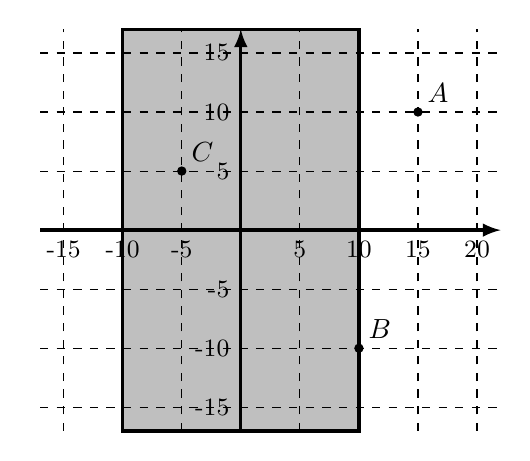
\begin{tikzpicture}[scale=0.15,>=latex]
    \draw [white] (-18,0) -- (-17,0) ;
    \fill [fill=gray!50] (-10,-17) rectangle (10,17) ;
    \draw [very thick] (-10,-17) rectangle (10,17) ;
    \draw [step=5,dashed] (-17,-17) grid (22,17) ;
    \foreach \x in {-15,-10,-5,5,10,15,20} {
      \draw [thick] (\x,0.1) -- (\x,-0.1) node [below] {\small \x} ;
    }
    \foreach \y in {-15,-10,-5,5,10,15} {
      \draw [thick] (0.1,\y) -- (-0.1,\y) node [left] {\small \y} ;
    }
    \node [fill,circle, inner sep=1.2pt] (A) at (15,10) {} ;
    \node at (A) [above right] {$A$} ;
    \node [fill,circle, inner sep=1.2pt] (B) at (10,-10) {} ;
    \node at (B) [above right] {$B$} ;
    \node [fill,circle, inner sep=1.2pt] (C) at (-5,5) {} ;
    \node at (C) [above right] {$C$} ;
    \draw [very thick,->] (-17,0) -- (22,0) ;
    \draw [very thick,->] (0,-17) -- (0,17) ;
  \end{tikzpicture}
}
\medskip

Ainsi, par exemple :
\begin{itemize}
  \item si la flèche atteint le point A, le tireur a raté la bande, et $X$
    prend la valeur $15$ ;
  \item si elle atteint le point B, l'impact est à la limite de la bande, et
    $X$ prend la valeur $10$ ;
  \item si elle atteint le point C, l'impact est dans la bande et $X$ prend
    la valeur $- 5$.
\end{itemize}

\medskip

On suppose que la variable aléatoire $X$ suit une loi normale d'espérance
$0$ et d'écart-type $10$.

\medskip

\begin{enumerate}
  \item Lorsque la flèche atteint le plan, déterminer la probabilité que son
    point d'impact soit situé hors de la bande grisée.
  \item  Comment modifier les bords de la bande grisée pour faire en sorte
    que, lorsque la flèche atteint le plan, son point d'impact soit situé à
    l'intérieur de la bande avec une probabilité égale à $0,6$ ?
\end{enumerate}

\bigskip

\textbf{Partie C}

\medskip

La durée de vie (exprimée en heures) du panneau électrique affichant le
score des concurrents est une variable aléatoire $T$ qui suit la loi
exponentielle de paramètre $\lambda = 10^{-4}$ (exprimé en
h$^{-1}$).

\medskip

\begin{enumerate}
  \item Quelle est la probabilité que le panneau fonctionne au moins pendant
    \np{2000}~heures ?
  \item \emph{Restitution organisée des connaissances}

    Dans cette question, $\lambda$ désigne un réel strictement positif.

    On rappelle que l'espérance mathématique de la variable aléatoire $T$
    suivant une loi exponentielle de paramètre $\lambda$, est définie par :
    E$(T) = \displaystyle\lim_{x \to + \infty} \displaystyle\int_0^x \lambda
    t \text{e}^{- \lambda t}\:\text{d}t$.
    \begin{enumerate}
      \item On considère la fonction $F$, définie pour tout réel $t$ par :
        $F(t) = \left(- t - \dfrac{1}{\lambda}\right)\text{e}^{- \lambda
        t}$.

        Démontrer que la fonction $F$ est une primitive sur $\R$ de la
        fonction $f$ définie pour tout réel $t$ par : $f(t) = \lambda
        t\text{e}^{- \lambda t}$.
      \item En déduire que l'espérance mathématique de la variable aléatoire
        $T$ est égale à $\dfrac{1}{\lambda}$.

        Quelle est l'espérance de durée de vie du panneau électrique
        affichant le score des
        concurrents ?
    \end{enumerate}
\end{enumerate}

\end{question}

\begin{question}[subtitle={Antilles Guyane 2015}]
\emph{La partie C peut être traitée indépendamment des parties A et B}

\bigskip

\textbf{Partie A}

\medskip

On considère une variable aléatoire $X$ qui suit la loi exponentielle de
paramètre $\lambda$ avec $\lambda > 0$.

On rappelle que, pour tout réel $a$ strictement positif,

\[P(X \leqslant  a) = \displaystyle\int_0^a \lambda\text{e}^{- \lambda
t}\:\text{d}t.\]

On se propose de calculer l'espérance mathématique de $X$, notée $E(X)$, et
définie par

\[E(X) = \displaystyle\lim_{x \to + \infty} \int_0^x \lambda t \text{e}^{-
\lambda t}\:\text{d}t.\]

On note $\R$ l'ensemble des nombres réels.

On admet que la fonction $F$ définie sur $\R$ par $F(t) = - \left(t +
\dfrac{1}{\lambda}\right)\text{e}^{- \lambda t}$ est une primitive sur $\R$
de la fonction $f$ définie sur $\R$ par $f(t) = \lambda t \text{e}^{-
\lambda t}$.

\medskip

\begin{enumerate}
  \item Soit $x$ un nombre réel strictement positif. Vérifier que

    \[\displaystyle \int_0^x \lambda t \text{e}^{- \lambda t}\:\text{d}t =
      \dfrac{1}{\lambda}\left(- \lambda x \text{e}^{- \lambda x} -
    \text{e}^{- \lambda x} + 1\right).\]

  \item  En déduire que $E(X) = \dfrac{1}{\lambda}$.
\end{enumerate}

\bigskip

\textbf{Partie B}

\medskip

La durée de vie, exprimée en années, d'un composant électronique peut être
modélisée par une variable aléatoire notée $X$ suivant la loi exponentielle
de paramètre $\lambda$ avec $\lambda > 0$.

La courbe de la fonction densité associée est représentée en \textbf{annexe 2}.

\medskip

\begin{enumerate}
  \item Sur le graphique de l'annexe 2 (à rendre avec la copie) :
    \begin{enumerate}
      \item Représenter la probabilité $P(X \leqslant  1)$.
      \item Indiquer où se lit directement la valeur de $\lambda$.
    \end{enumerate}
  \item  On suppose que $E(X) = 2$.
    \begin{enumerate}
      \item Que représente dans le cadre de l'exercice la valeur de
        l'espérance mathématique de la variable aléatoire $X$ ?
      \item Calculer la valeur de $\lambda$.
      \item Calculer $P(X \leqslant 2)$. On donnera la valeur exacte puis la
        valeur arrondie à $0,01$ près.

        Interpréter ce résultat.
      \item Sachant que le composant a déjà fonctionné une année, quelle est
        la probabilité que sa durée de vie totale soit d'au moins trois
        années ? On donnera la valeur exacte.
    \end{enumerate}
\end{enumerate}

\bigskip

\textbf{Partie C}

\medskip

Un circuit électronique est composé de deux composants identiques numérotés 1 et 2.
On note $D_1$ l'évènement \og le composant 1 est défaillant avant un an
\fg{} et on note $D_2$ l'évènement \og le composant 2 est défaillant avant
un an \fg.

On suppose que les deux évènements $D_1$ et $D_2$ sont indépendants et que 

$P\left(D_1\right) = P\left(D_2\right) = 0,39$.

Deux montages possibles sont envisagés, présentés ci-dessous :

\begin{center}
  \begin{tikzpicture}
    \draw (0,0) -- (1,0) -- (1,1) -- (2,1) node
    [rectangle,fill=white,draw,inner sep=2pt,text width=1cm]
    {\hfill 1\hfill~} -- (3,1) -- (3,0) -- (4,0) ;
    \draw (0,0) -- (1,0) -- (1,-1) -- (2,-1) node
    [rectangle,fill=white,draw,inner sep=2pt,text width=1cm]
    {\hfill 2\hfill~} -- (3,-1) -- (3,0) -- (4,0) ;
    \draw (5+0,0) -- (5+5,0) ;
    \draw (5+1.7,0) node
    [rectangle,fill=white,draw,inner sep=2pt,text width=1cm]
    {\hfill 1\hfill~} ;
    \draw (5+3.2,0) node
    [rectangle,fill=white,draw,inner sep=2pt,text width=1cm]
    {\hfill 2\hfill~} ;
    \draw (2,-2) node {Circuit en parallèle} ;
    \draw (5+2,-2) node {Circuit en série} ;
  \end{tikzpicture}
\end{center}

\medskip

\begin{enumerate}
  \item Lorsque les deux composants sont montés \og en parallèle \fg, le
    circuit A est défaillant uniquement si les deux composants sont
    défaillants en même temps. Calculer la probabilité que le circuit A soit
    défaillant avant un an.
  \item Lorsque les deux composants sont montés \og en série \fg, le circuit
    B est défaillant dès que l'un au moins des deux composants est
    défaillant. Calculer la probabilité que le circuit B soit défaillant
    avant un an.
\end{enumerate}

\begin{center}
  \begin{tikzpicture}[xscale=1.41,yscale=14.1,>=latex]
    \draw [xstep=1,ystep=0.1,dashed,gray] (0,0) grid (10,0.7) ;
    \draw [thick, blue] plot [smooth,domain=0:10] (\x,{0.5*exp(-\x/2) }) ;
    \draw [very thick,->] (0,0) -- (10.3,0) ;
    \draw [very thick,->] (0,0) -- (0,0.7) ;
    \foreach \x in {0,1,...,10} {
      \draw [thick] (\x,0.01) -- (\x,-0.01) node [below] {\x} ;
    }
    \foreach \y in {0,0.1,0.2,0.3,0.4,0.5,0.6} {
      \draw [thick] (0.1,\y) -- (-0.1,\y) node [left] {\np{\y}} ;
    }
    \draw (0,0.7) node [left] {$y$} ; \draw (10.3,0) node [below] {$x$} ;
  \end{tikzpicture}
\end{center}

\end{question}

\begin{question}[subtitle={Métropole 2015}]
\emph{Les résultats des probabilités seront arrondis à $10^{-3}$ près.}

\bigskip

\textbf{Partie 1}

\medskip

\begin{enumerate}
\item Soit $X$ une variable aléatoire qui suit la loi exponentielle de paramètre $\lambda$, où $\lambda$ est un réel strictement positif donné.

On rappelle que la densité de probabilité de cette loi est la fonction $f$  définie sur
$[0~;~+ \infty[$ par
\[f(x) = \lambda\text{e}^{- \lambda x}.\]

\begin{enumerate}
  \item Soit $c$ et $d$ deux réels tels que $0 \leqslant c < d$.

Démontrer que la probabilité $P( c \leqslant X \leqslant d)$ vérifie 

$P(c \leqslant X \leqslant d) = \text{e}^{- \lambda c}   - \text{e}^{- \lambda d}$.
    \item Déterminer une valeur de $\lambda$ à $10^{-3}$ près de telle sorte
      que la probabilité $P(X > 20)$ soit égale à 0,05.
    \item Donner l'espérance de la variable aléatoire $X$

\medskip

\textbf{Dans la suite de l'exercice on prend } \boldmath$\lambda = 0,15$\unboldmath.
    \item Calculer $P(10 \leqslant X \leqslant 20)$.
    \item Calculer la probabilité de l'évènement $(X > 18)$.
  \end{enumerate}
\item Soit $Y$ une variable aléatoire qui suit la loi normale d'espérance $16$ et d'écart type $1,95$.\index{loi normale}
  \begin{enumerate}
    \item Calculer la probabilité de l'évènement $(20 \leqslant Y \leqslant 21)$.
    \item Calculer la probabilité de l'évènement $(Y < 11) \cup (Y > 21)$.
  \end{enumerate}
\end{enumerate}

\bigskip

\textbf{Partie 2}

\medskip

Une chaîne de magasins souhaite fidéliser ses clients en offrant des bons
d'achat à ses clients privilégiés. Chacun d'eux reçoit un bon d'achat de
couleur verte ou rouge sur lequel est inscrit un montant.

Les bons d'achats sont distribués de façon à avoir, dans chaque magasin, un
quart de bons rouges et trois quarts de bons verts.

Les bons d'achat verts prennent la valeur de $30$~euros avec une probabilité
égale à $0,067$ ou des valeurs comprises entre $0$ et $15$~euros avec des
probabilités non précisées ici.

De façon analogue, les bons d'achat rouges prennent les valeurs $30$ ou
$100$~euros avec des probabilités respectivement égales à $0,015$ et $0,010$
ou des valeurs comprises entre $10$ et $20$~euros avec des probabilités non
précisées ici.

\medskip

\begin{enumerate}
  \item Calculer la probabilité d'avoir un bon d'achat d'une valeur
    supérieure ou égale à $30$~euros sachant qu'il est rouge.
  \item Montrer qu'une valeur approchée à $10^{-3}$ près de la probabilité
    d'avoir un bon d'achat d'une valeur supérieure ou égale à $30$~euros
    vaut $0,057$.

    \textbf{Pour la question suivante, on utilise cette valeur.}

  \item Dans un des magasins de cette chaîne, sur $200$ clients privilégiés, $6$ ont reçu un bon d'achat d'une valeur supérieure ou égale à $30$~\euro.

    \smallskip

    Le directeur du magasin considéré estime que ce nombre est insuffisant
    et doute de la répartition au hasard des bons d'achats dans les
    différents magasins de la chaîne.

    Ses doutes sont-ils justifiés ?
\end{enumerate}

\end{question}

\begin{question}[subtitle={Métropole septembre 2015}]
\emph{Cet exercice est un questionnaire à choix multiples. Pour chacune des questions, quatre réponses sont proposées, dont une seule est exacte. Le candidat portera sur la copie le numéro de la question suivi de la réponse choisie. On ne demande pas de justification. Il est attribué $1$ point si la réponse est exacte. Aucun point n'est enlevé en l'absence de réponse ou en cas de réponse fausse.}\index{Q. C. M.}

\medskip

\textbf{Question 1}

\parbox{0.6\linewidth}{On considère l'arbre de probabilités ci-contre :}\hfill
%\parbox{0.4\linewidth}{\psset{unit=1.5cm}
%\pstree[treemode=R,nodesepB=4pt]{\TR{}}
%{
%	\pstree[nodesepA=4pt]{\TR{$A$}\ncput*{0,6}}
%	  { 
%		  \TR{$B$}\ncput*{0,2}
%		  \TR{$\overline{B}$}	   
%	  }
%	\pstree[nodesepA=4pt]{\TR{$\overline{A}$}}
%	  {
%		  \TR{$B$}\ncput*{0,3}
%		  \TR{$\overline{B}$}
%	  }
%}
%}\index{arbre de probabilités}
\medskip

Quelle est la probabilité de l'évènement $B$ ?

\medskip
\begin{tabularx}{\linewidth}{*{4}{X}}
\textbf{a.~~} 0,12&\textbf{b.~~} 0,2&\textbf{c.~~} 0,24 &\textbf{d.~~} 0,5
\end{tabularx}
\medskip

\textbf{Question 2}

Le césium 137 est un élément radioactif qui constitue une des principales sources de radioactivité des déchets des réacteurs nucléaires. Le temps $T$, en années, durant lequel un atome de césium 137 reste radioactif peut être assimilé à une variable aléatoire $T$ qui suit la loi exponentielle de paramètre $\lambda = \dfrac{\ln 2}{30}$.\\[5pt]
Quelle est la probabilité qu'un atome de césium 137 reste radioactif durant au moins 60 ans ?\index{loi exponentielle}

\medskip
\begin{tabularx}{\linewidth}{*{4}{X}}
\textbf{a.~~} 0,125&\textbf{b.~~} 0,25&\textbf{c.~~} 0,75 &\textbf{d.~~} 0,875
\end{tabularx}
\medskip

\textbf{Question 3}

Soit $X$ une variable aléatoire qui suit la loi normale d'espérance $\mu = 110$ et d'écart-type $\sigma = 25$.\index{loi normale}

Quelle est la valeur arrondie au millième de la probabilité $P( X \geqslant 135)$ ?

\medskip
\begin{tabularx}{\linewidth}{*{4}{X}}
\textbf{a.~~} 0,159&\textbf{b.~~} 0,317 &\textbf{c.~~} 0,683 &\textbf{d.~~} 0,841
\end{tabularx}
\medskip
\end{question}

\begin{question}[subtitle={Polynésie septembre 2015}]
On étudie une maladie dans la population d'un pays. On a constaté que le taux, en nanogrammes
par millilitre $\left(\text{ng.mL}^{-1}\right)$, d'une substance Gamma présente dans le sang est plus élevé chez les personnes atteintes de cette maladie que chez les personnes qui n'en sont pas
atteintes.

\medskip

\begin{enumerate}
\item Le taux de cette substance Gamma dans la population des personnes qui ne sont pas
atteintes par la maladie est modélisé par une variable aléatoire $T$ qui suit la loi normale
d'espérance $\mu = 40$ et d'écart-type $\sigma = 8$.\index{loi normale}

On choisit au hasard une personne parmi celles qui ne sont pas atteintes par la maladie
étudiée.

Calculer la probabilité que le taux dans le sang de la substance Gamma soit supérieur
à 60 ng.mL$^{-1}$.
\item Des études ont mis en évidence que le taux moyen de la substance Gamma chez les
personnes atteintes par la maladie étudiée est de 50 ng.mL$^{-1}$ et que 10\,\% d'entre elles
ont un taux de substance Gamma inférieur à 43 ng.mL$^{-1}$.

On appelle $T'$ la variable aléatoire qui modélise le taux de la substance Gamma en
ng.mL$^{-1}$ chez une personne atteinte par la maladie étudiée.

On admet que $T'$ suit la loi normale d'espérance $\mu'$ et d'écart-type $\sigma'$.\index{loi normale}

Préciser la valeur de $\mu'$ et déterminer la valeur de $\sigma'$.
\end{enumerate}
\end{question}

\begin{question}[subtitle={Antilles Guyane septembre 2015}]
Dans un supermarché, on réalise une étude sur la vente de bouteilles de jus de fruits sur une période d'un mois.

\setlength\parindent{8mm}
\begin{itemize}
\item[$\bullet~~$]40\,\% des bouteilles vendues sont des bouteilles de jus d'orange ;
\item[$\bullet~~$]25\,\% des bouteilles de jus d'orange vendues possèdent l'appellation \og pur jus \fg.
\end{itemize}
\setlength\parindent{0mm} 

\medskip

Parmi les bouteilles qui ne sont pas de jus d'orange, la proportion des bouteilles de \og pur jus \fg{} est notée $x$, où $x$ est un réel de l'intervalle [0~;~1].

Par ailleurs, 20\,\% des bouteilles de jus de fruits vendues possèdent l'appellation \og pur jus \fg.

On prélève au hasard une bouteille de jus de fruits passée en caisse. On définit les évènements suivants :\index{probabilités}

$R$ : la bouteille prélevée est une bouteille de jus d'orange ;

$J$ : la bouteille prélevée est une bouteille de \og pur jus \fg.

\bigskip

\textbf{Partie A}

\medskip

\begin{enumerate}
\item Représenter cette situation à l'aide d'un arbre pondéré.\index{arbre de probabilités}
\item Déterminer la valeur exacte de $x$.
\item Une bouteille passée en caisse et prélevée au hasard est une bouteille de \og pur jus \fg.

Calculer la probabilité que ce soit une bouteille de jus d'orange.
\end{enumerate}

\bigskip

\textbf{Partie B}

\medskip

Afin d'avoir une meilleure connaissance de sa clientèle, le directeur du supermarché fait une étude sur un lot des $500$ dernières bouteilles de jus de fruits vendues.

On note $X$ la variable aléatoire égale au nombre de bouteilles de \og pur jus \fg{} dans ce lot.

On admettra que le stock de bouteilles présentes dans le supermarché est suffisamment important pour que le choix de ces $500$ bouteilles puisse être assimilé à un tirage au sort avec remise.

\medskip

\begin{enumerate}
\item Déterminer la loi suivie par la variable aléatoire $X$. On en donnera les paramètres.
\item Déterminer la probabilité pour qu'au moins 75 bouteilles de cet échantillon de $500$ bouteilles soient de \og pur jus \fg. On arrondira le résultat au millième.
\end{enumerate}

\bigskip

\end{question}

\end{document}
